
\section{Measurement of SF for the Single Electron Trigger}

\subsection{Measurement Approach}

Single electron trigger, \texttt{HLT\_Ele27\_WPTight\_Gsf}, is used in the $ee$, $e\mu$, $e\tau_h$, $e+jets$ channels.
In shape analysis, since the fitted template in $ee$ and $e+jets$ is based on the $p^T_e$ spectra, a pt dependent 
uncertainty of scale factors of \texttt{HLT\_Ele27\_WPTight\_Gsf} efficiency is needed to account for the trigger 
systematics properly of the templates of $p^T_e$ spectra. Here a customized measurement of scale factor and the 
associated uncertainties
of \texttt{HLT\_Ele27\_WPTight\_Gsf} trigger is performed based on 2016 re-reco dataset with the tag-prob approach. 
The uncertainty
of the scale factor includes both statistical and systematical uncertainty, where systematical uncertainty are estimated by
"two shifts":

\begin{itemize}
  \item shift up the tagging electron by 10 GeV to effectively simulate a different trigger. This estimates the 
  systematical effect that some L1 seed could have a threshold of 32 GeV.
  \item shift the probing electron pT up and down by 0.5 GeV. This estimates the effect of the electron \pt resolution.
\end{itemize}

The dataset used in the measurement is 2016 re-reco dataset \texttt{ SingleElectron/Run2016[B-H]-03Feb2017-*}
with the golden certificate as luminosity mask. The mc simulations used in the measurement are 
\begin{itemize}
    \item \texttt{DYJETSToLL\_M-10to50\_amcatnlo},
    \item \texttt{DYJETSToLL\_M-50\_amcatnlo},
    \item \texttt{TT\_powheg},
\end{itemize}
\noindent in which events reweighted to pile-up $\sigma_{mb} = 69.2\pm 2.3 mb$.

A standard tag-prob method is used in the measurement of the scale factor of the trigger efficiency.
The electrons are selected with tight id and tight PF isolation with $p^T_e>20$ GeV and $|\eta_e|<2.5$. Corrections
to the electrons in the MC simulation includes energy scale-smear, reconstruction and isolation. 
Among selected electrons, tagged electrons
are defined as $p^T_e>30$ GeV and outside gap between barrel and endcap caolritmeters $1.444<|\eta_e|<1.56$, and 
match with \texttt{HLT\_Ele27\_WPTight\_Gsf} triggering objects. Events are selected by requiring exactly 2
opposite electrons with at least 1 tagged electron and $60<m_{ee}<120$ GeV. This event selection yields a set of events 
significantly dominated by Drell-Yan process. The distribution of $m_{ee}$ is shown in fig~\ref{fig:appendix:ele27TriggerSF}.
The purity of Drell-Yan are very high in the selected events. Thus a signal-backgound fit is not necessary to get DY yields.



\begin{figure}
    \centering
    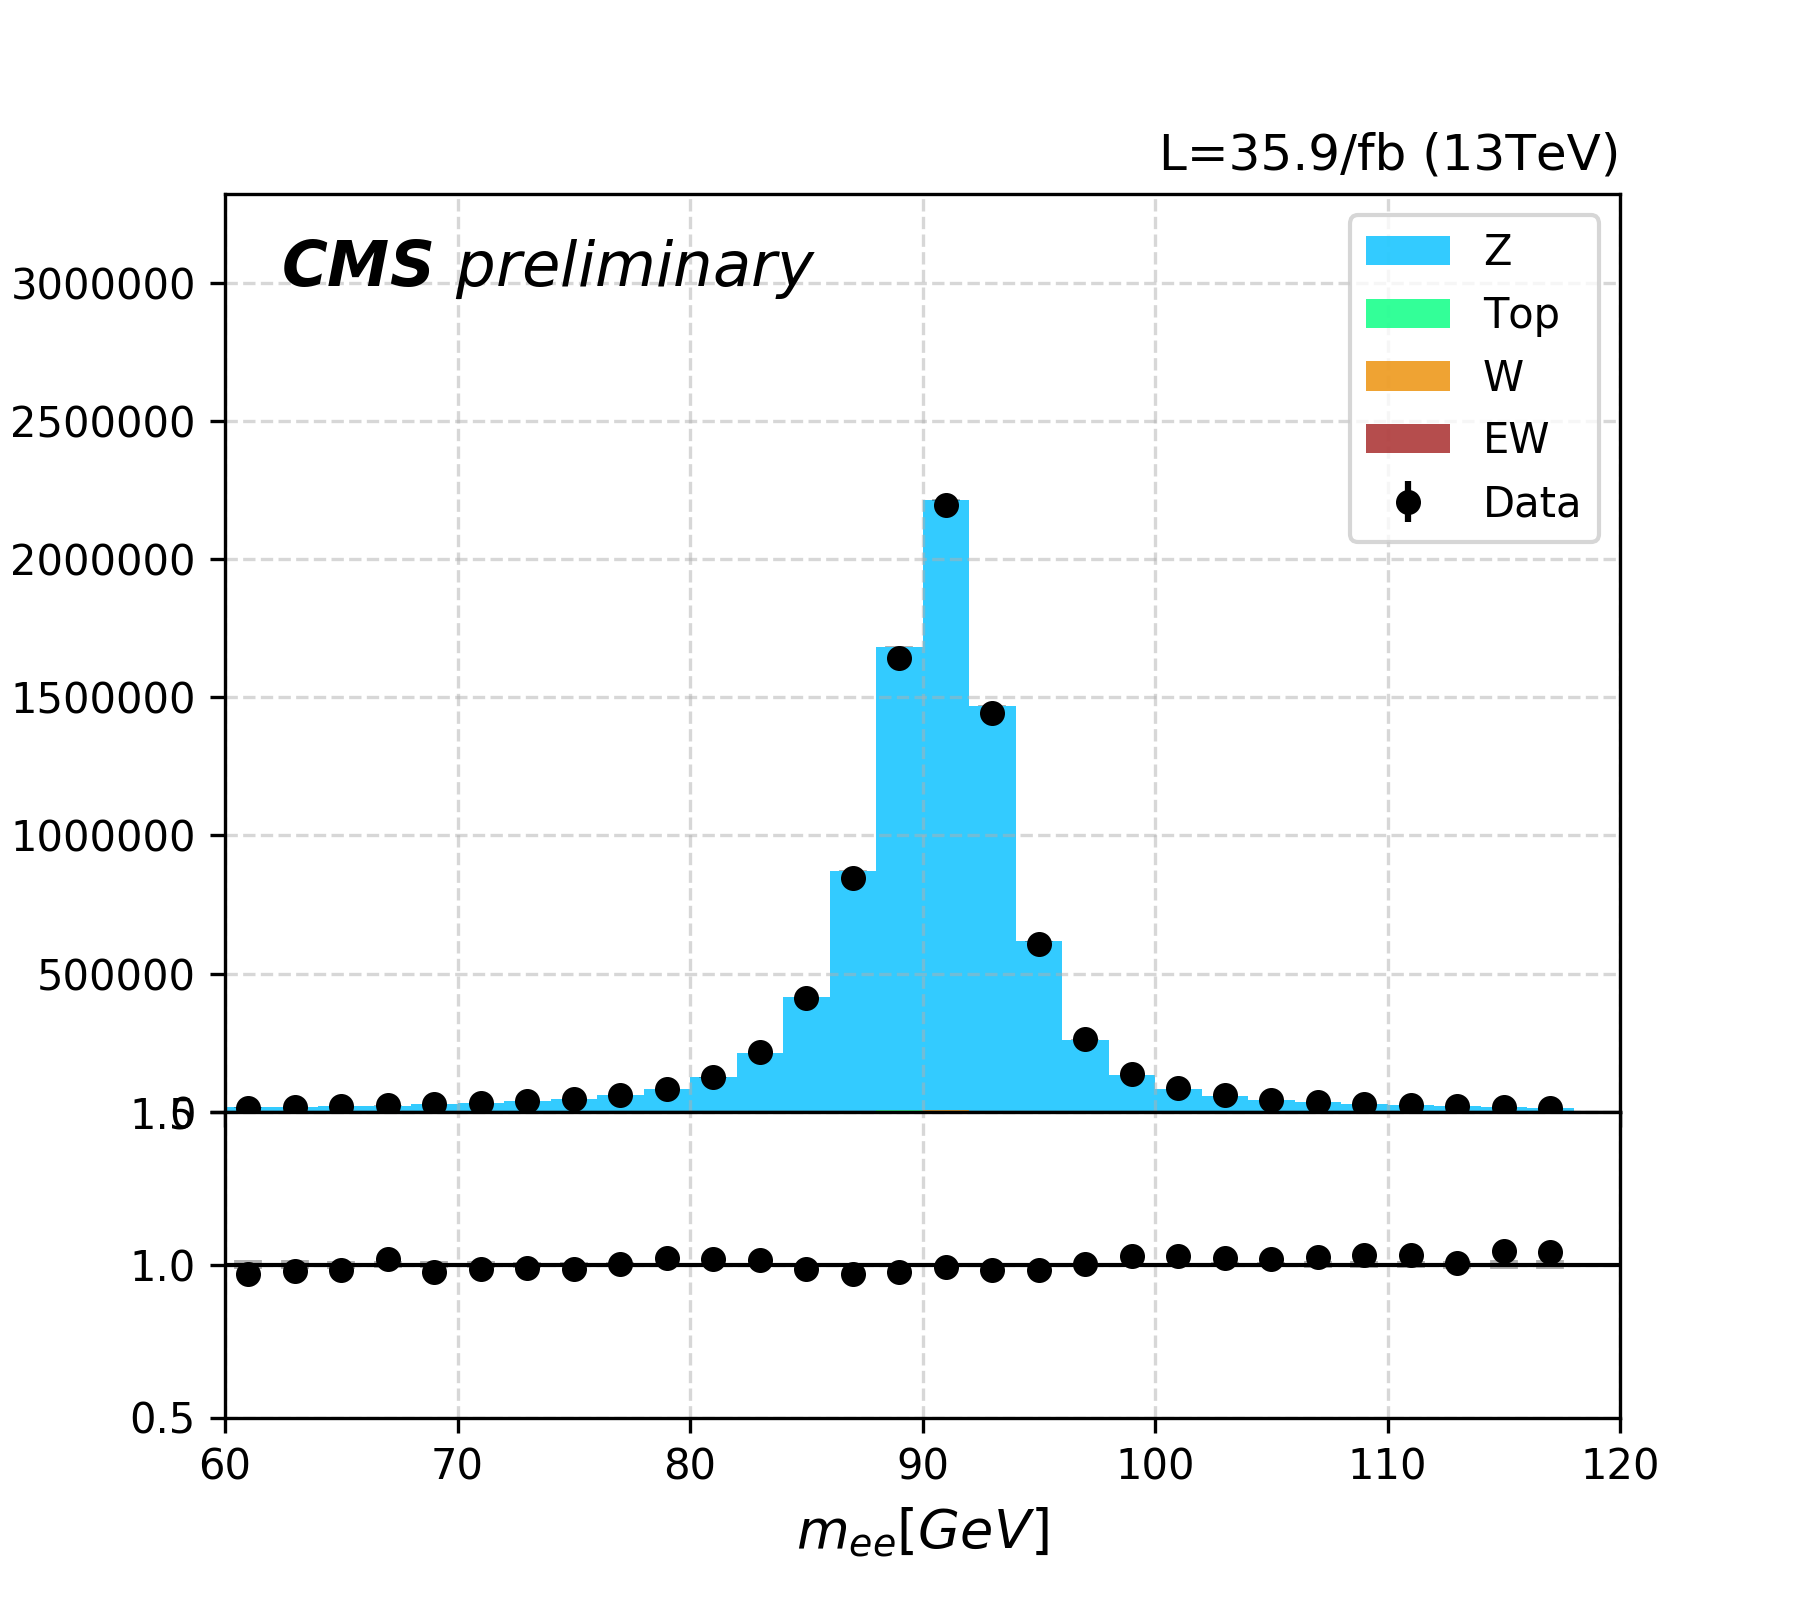
\includegraphics[width=0.6\textwidth]{chapters/Appendix/sectionEleTrigger/figures/dileptonMass_tag30.png}
    \caption{$m_{ee}$ of the selected events for the measurement of the $SF$ trigger efficiency.}
    \label{fig:appendix:ele27TriggerSF}
\end{figure}

In each event, if one electron is tagged, the other become a prob. Each event provides eigher 1 or 2 tag-prob pairs.
A prob is passing if it match with \texttt{HLT\_Ele27\_WPTight\_Gsf} triggering objects.
The trigger efficiencies are calculated by the ratio between the number of passing probs and total probs in each $p^T_e-\eta_e$ bin, 

\begin{equation}
    \epsilon (\pt, \eta) = \frac{ N_{\rm passing} (\pt, \eta) } {  N_{\rm total} (\pt, \eta) }.
\end{equation}

\noindent The scale factors are derived by taking the ratio between efficiencies of data over MC,
\begin{equation}
SF (\pt, \eta) = \frac{\epsilon_{\rm{data}} (\pt, \eta) }{\epsilon_{\rm{MC}} (\pt, \eta) }.
\end{equation}



\subsection{Result of the SF and the uncertainties}

In 2016 B-F, the data efficiency in the endcap decreases because there is a decrease of signal over noise ratio associated 
to loss of	tracking hits caused by problems in the pre-amplifier of the APV chip. 
In the mid August 2016, this problem of Si-strip in endcap region is fixed by increase the drain speed of the pre-amplifier. Thus the 
trigger efficiencies are improved in 2016 GH. So the measurement of the scale factor of the trigger efficiency is divided into to
two parts based on data taking periods, the 2016 B-F and 2016 GH.

The 2D maps of $\epsilon_{\rm{data}}$, $\epsilon_{\rm{MC}}$ and $SF$ in both 2016 B-F and 2016 GH are shown in Figure~\ref{fig:appendix:ele27SF}. Figure~\ref{fig:appendix:ele27SFperiods} 
shows the $SF$ in each 2016 data taking period, where the improvement in the G period is clear.



\begin{figure}
    \centering
    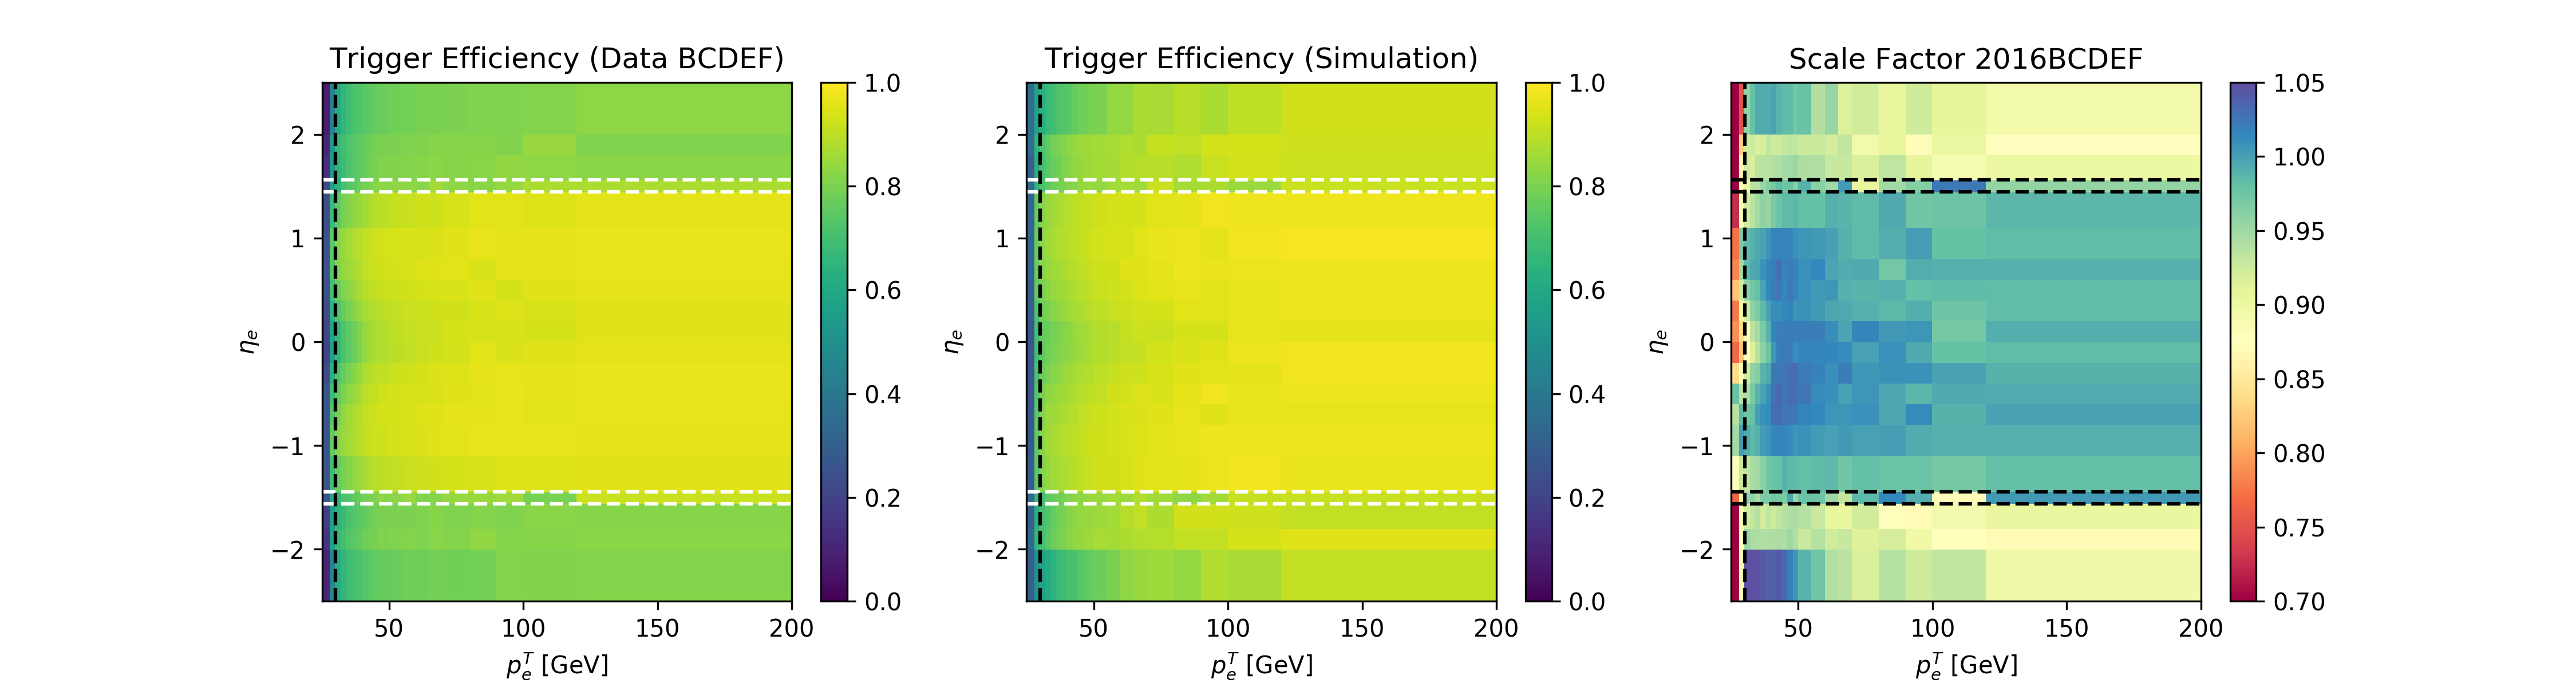
\includegraphics[width=0.99\textwidth]{chapters/Appendix/sectionEleTrigger/figures/eff2d_BCDEF.png}
    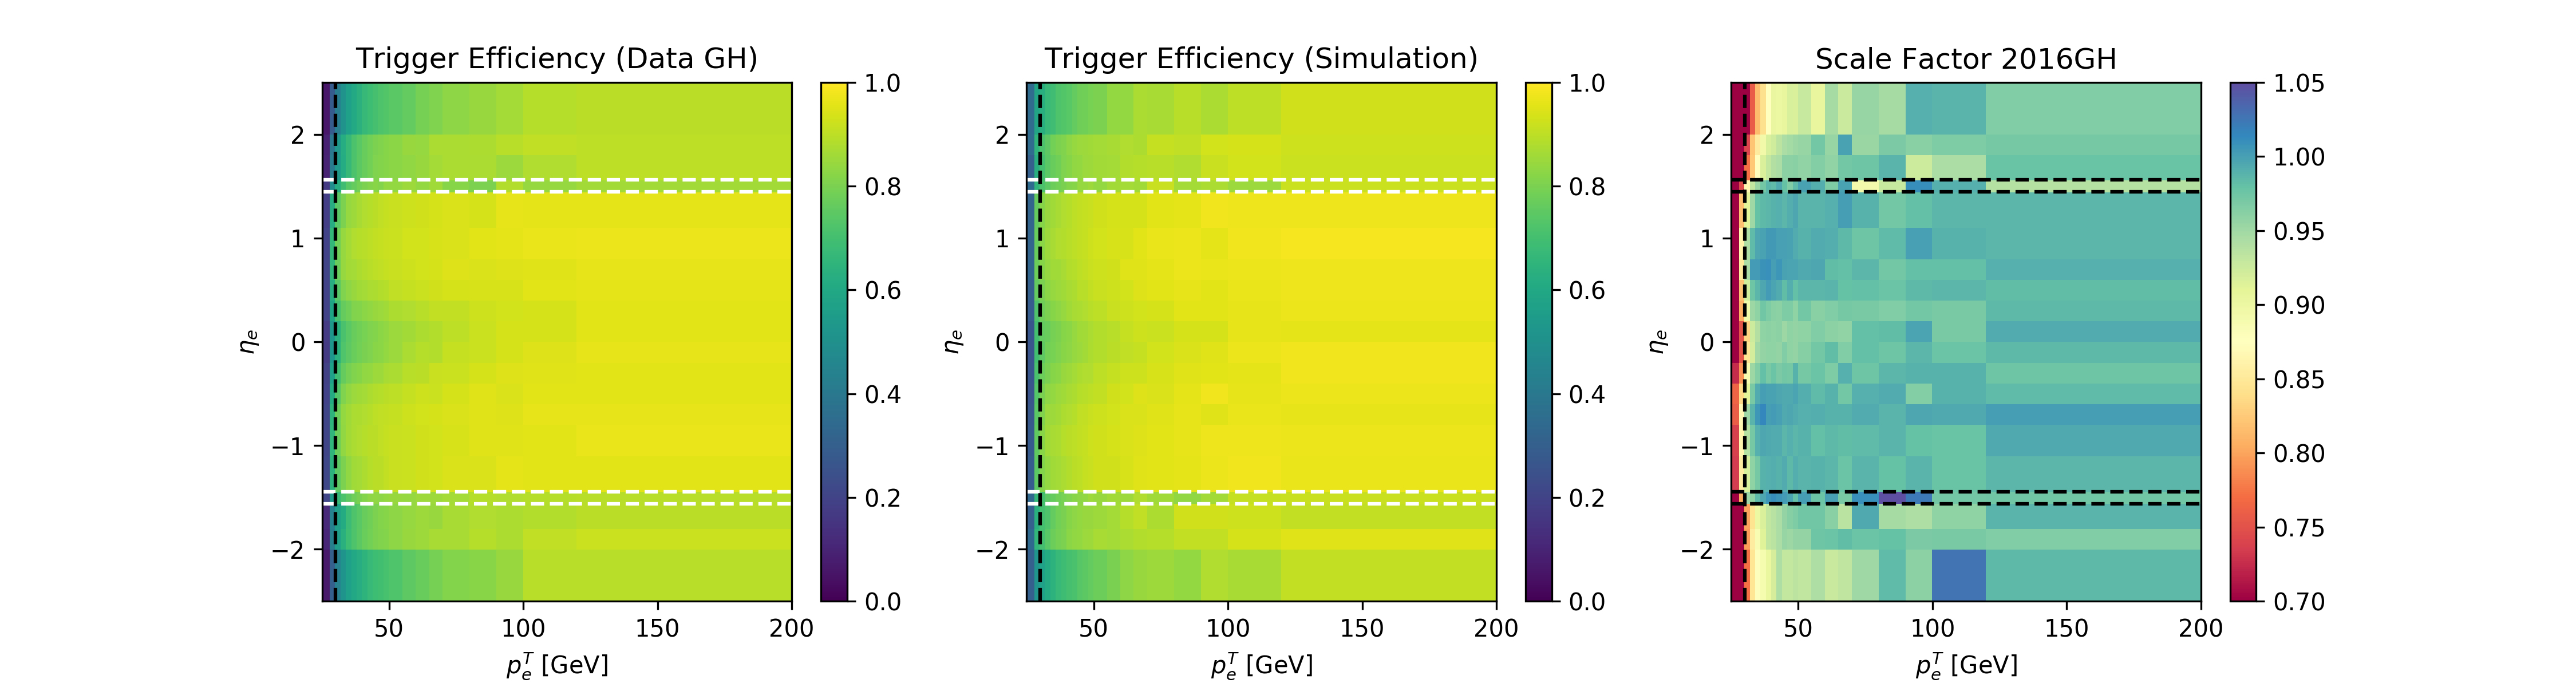
\includegraphics[width=0.99\textwidth]{chapters/Appendix/sectionEleTrigger/figures/eff2d_GH.png}
    \caption{The 2D maps of $\epsilon_{\rm{data}}$, $\epsilon_{\rm{MC}}$ and $SF$ in both 2016 B-F and 2016 GH.}
    \label{fig:appendix:ele27SF}
\end{figure}



\begin{figure}
    \centering
    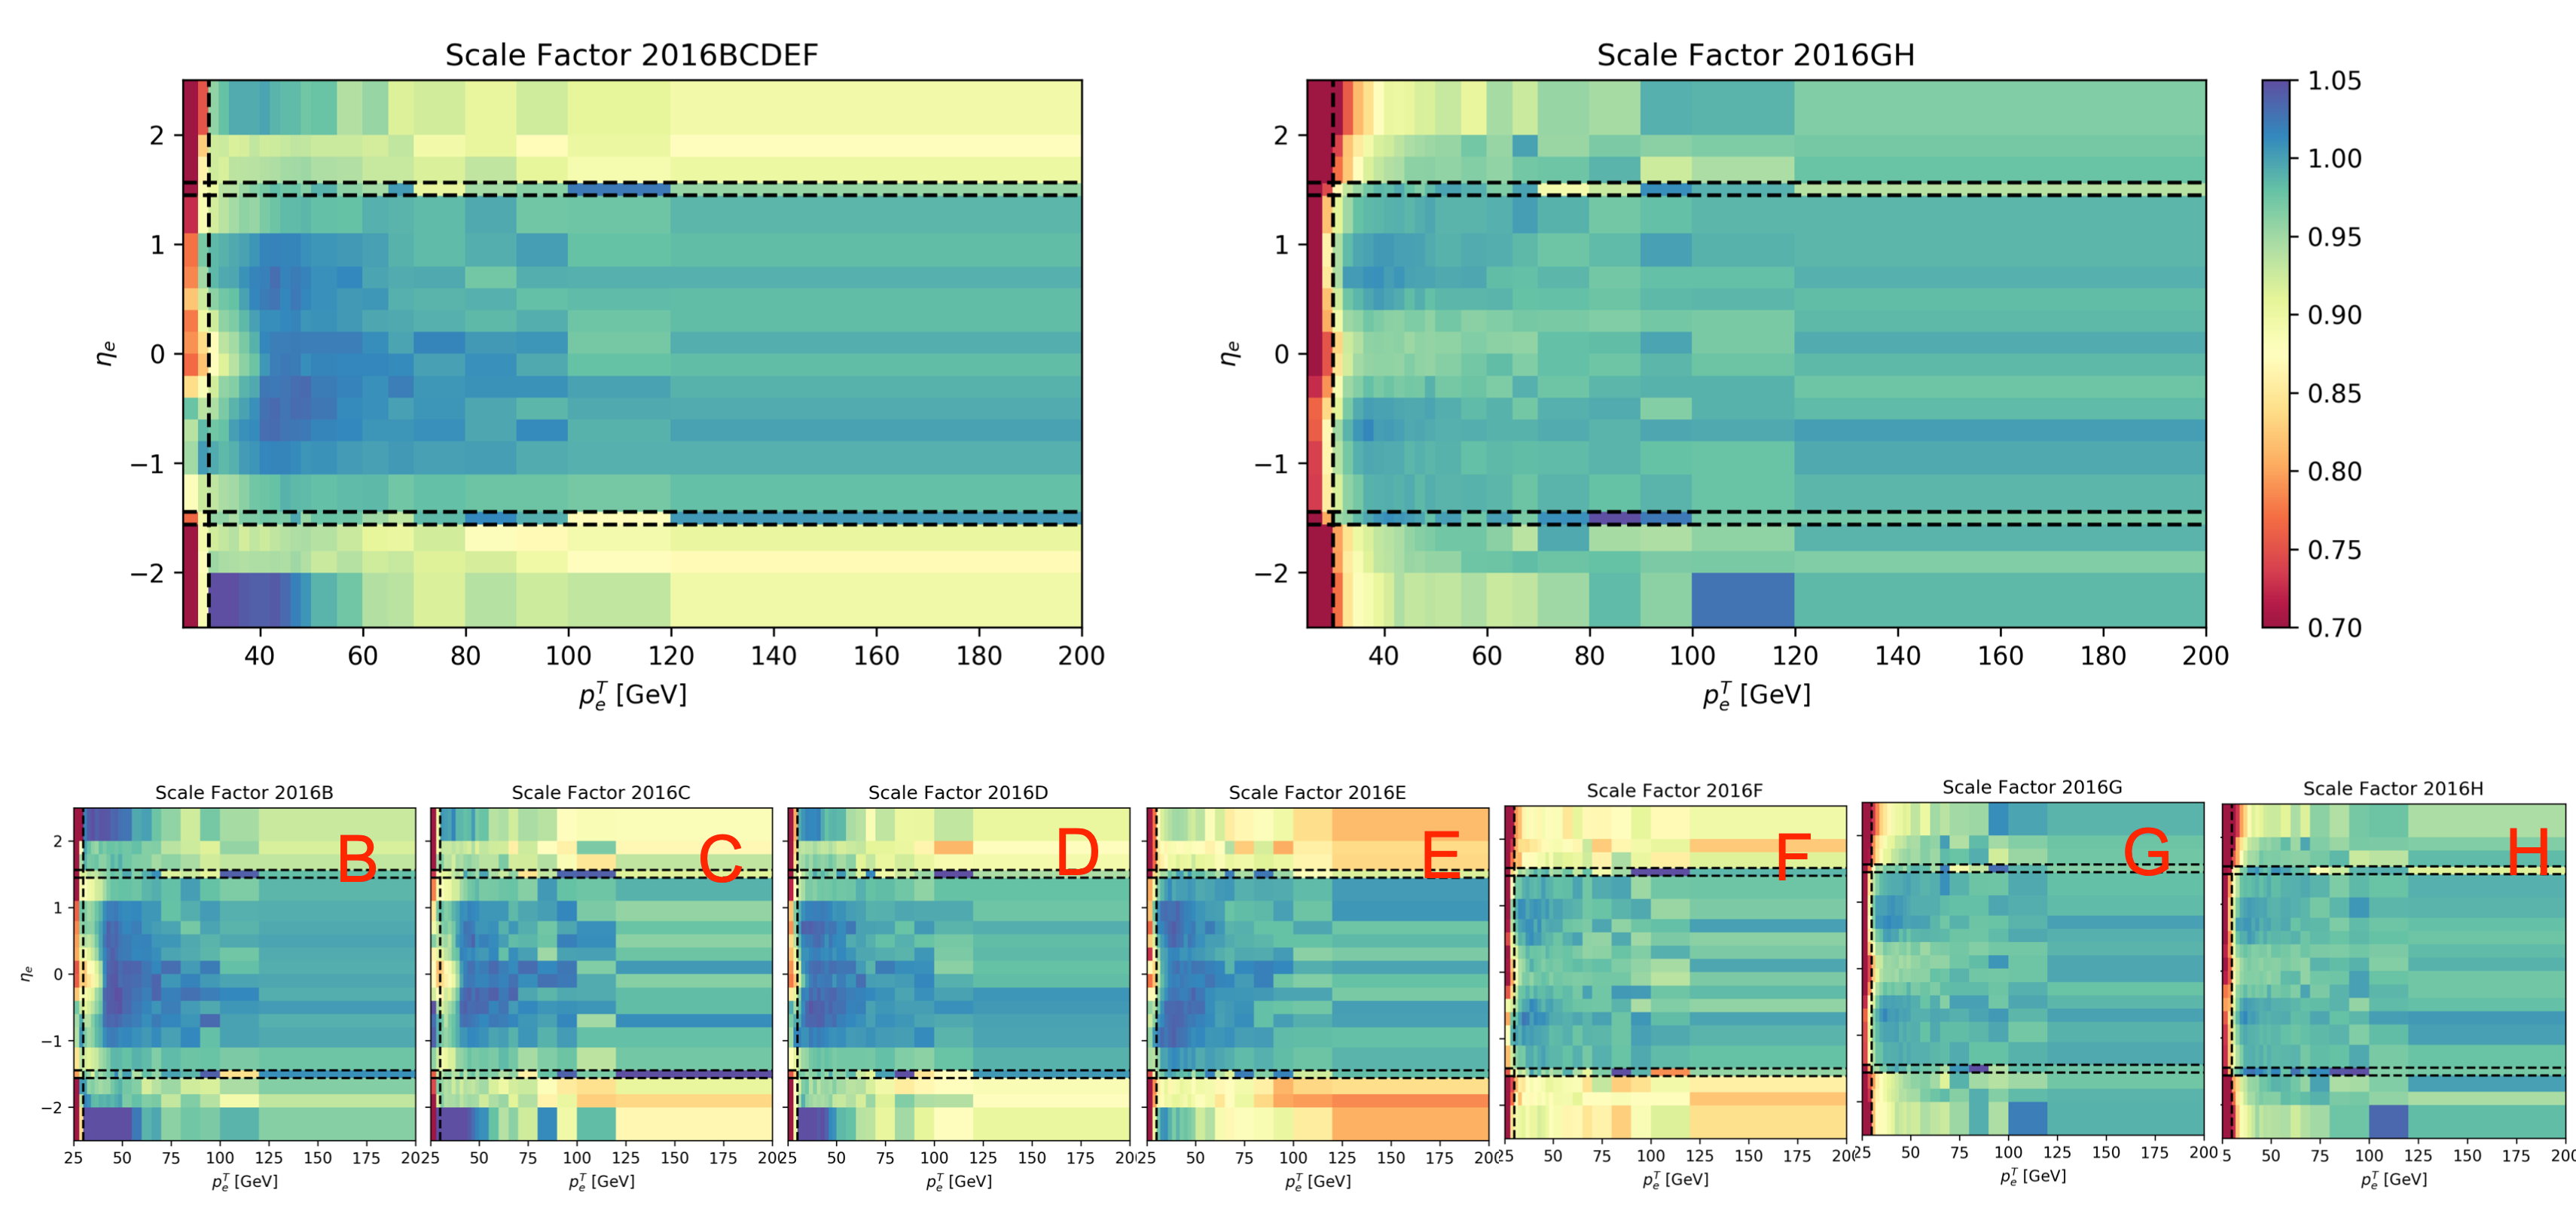
\includegraphics[width=0.99\textwidth]{chapters/Appendix/sectionEleTrigger/figures/eTrSF_value.png}
    \caption{$SF$ in each 2016 data taking period.}
    \label{fig:appendix:ele27SFperiods}
\end{figure}





For the two parts, 2016 B-F and GH, the systematical uncertainties are estimated by the "two shifts" approach described above. 
The total uncertainty combines the statistical and systematical uncertainties from tag and prob "two shifts".
The final result of the SF and the associated uncertainties are shown in fig~\ref{fig:eTrSF_err_BCDEF} and \ref{fig:eTrSF_err_GH}.

\begin{figure}
    \centering
    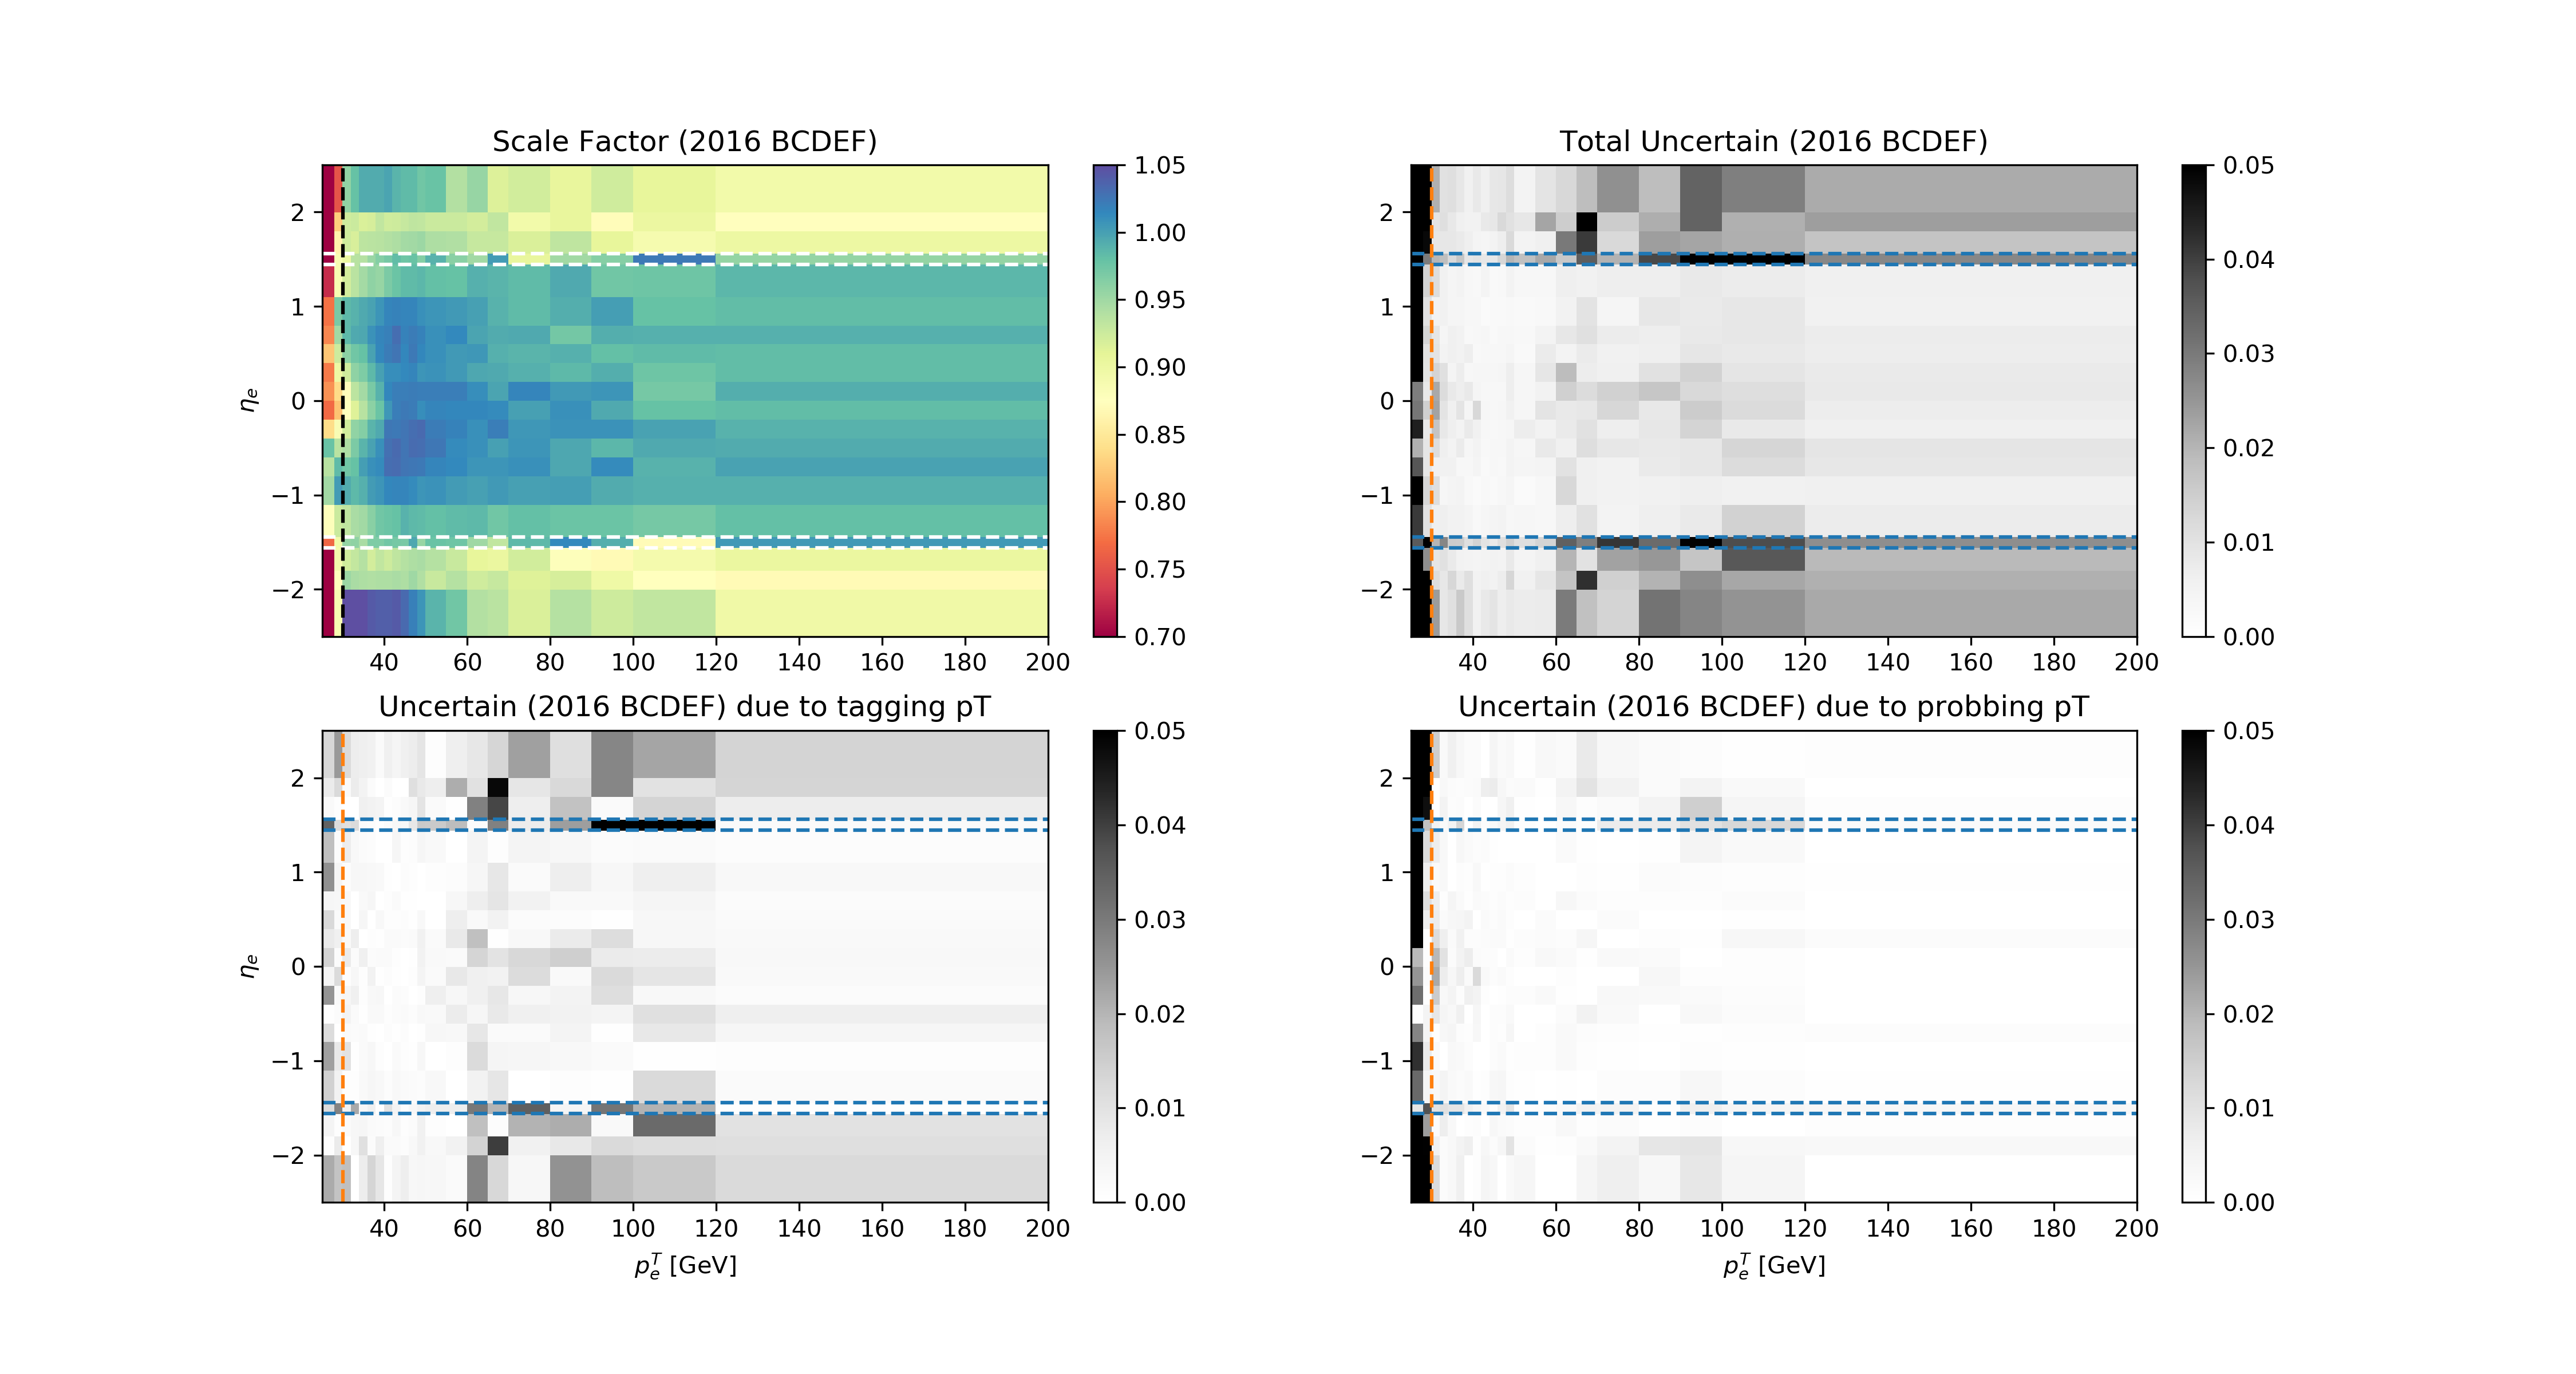
\includegraphics[width=0.99\textwidth]{chapters/Appendix/sectionEleTrigger/figures/result_BCDEF.png}
    
    \caption{SF and the associated uncertainties in the 2016 B-F.}
    \label{fig:eTrSF_err_BCDEF}
\end{figure}

\begin{figure}
    \centering
    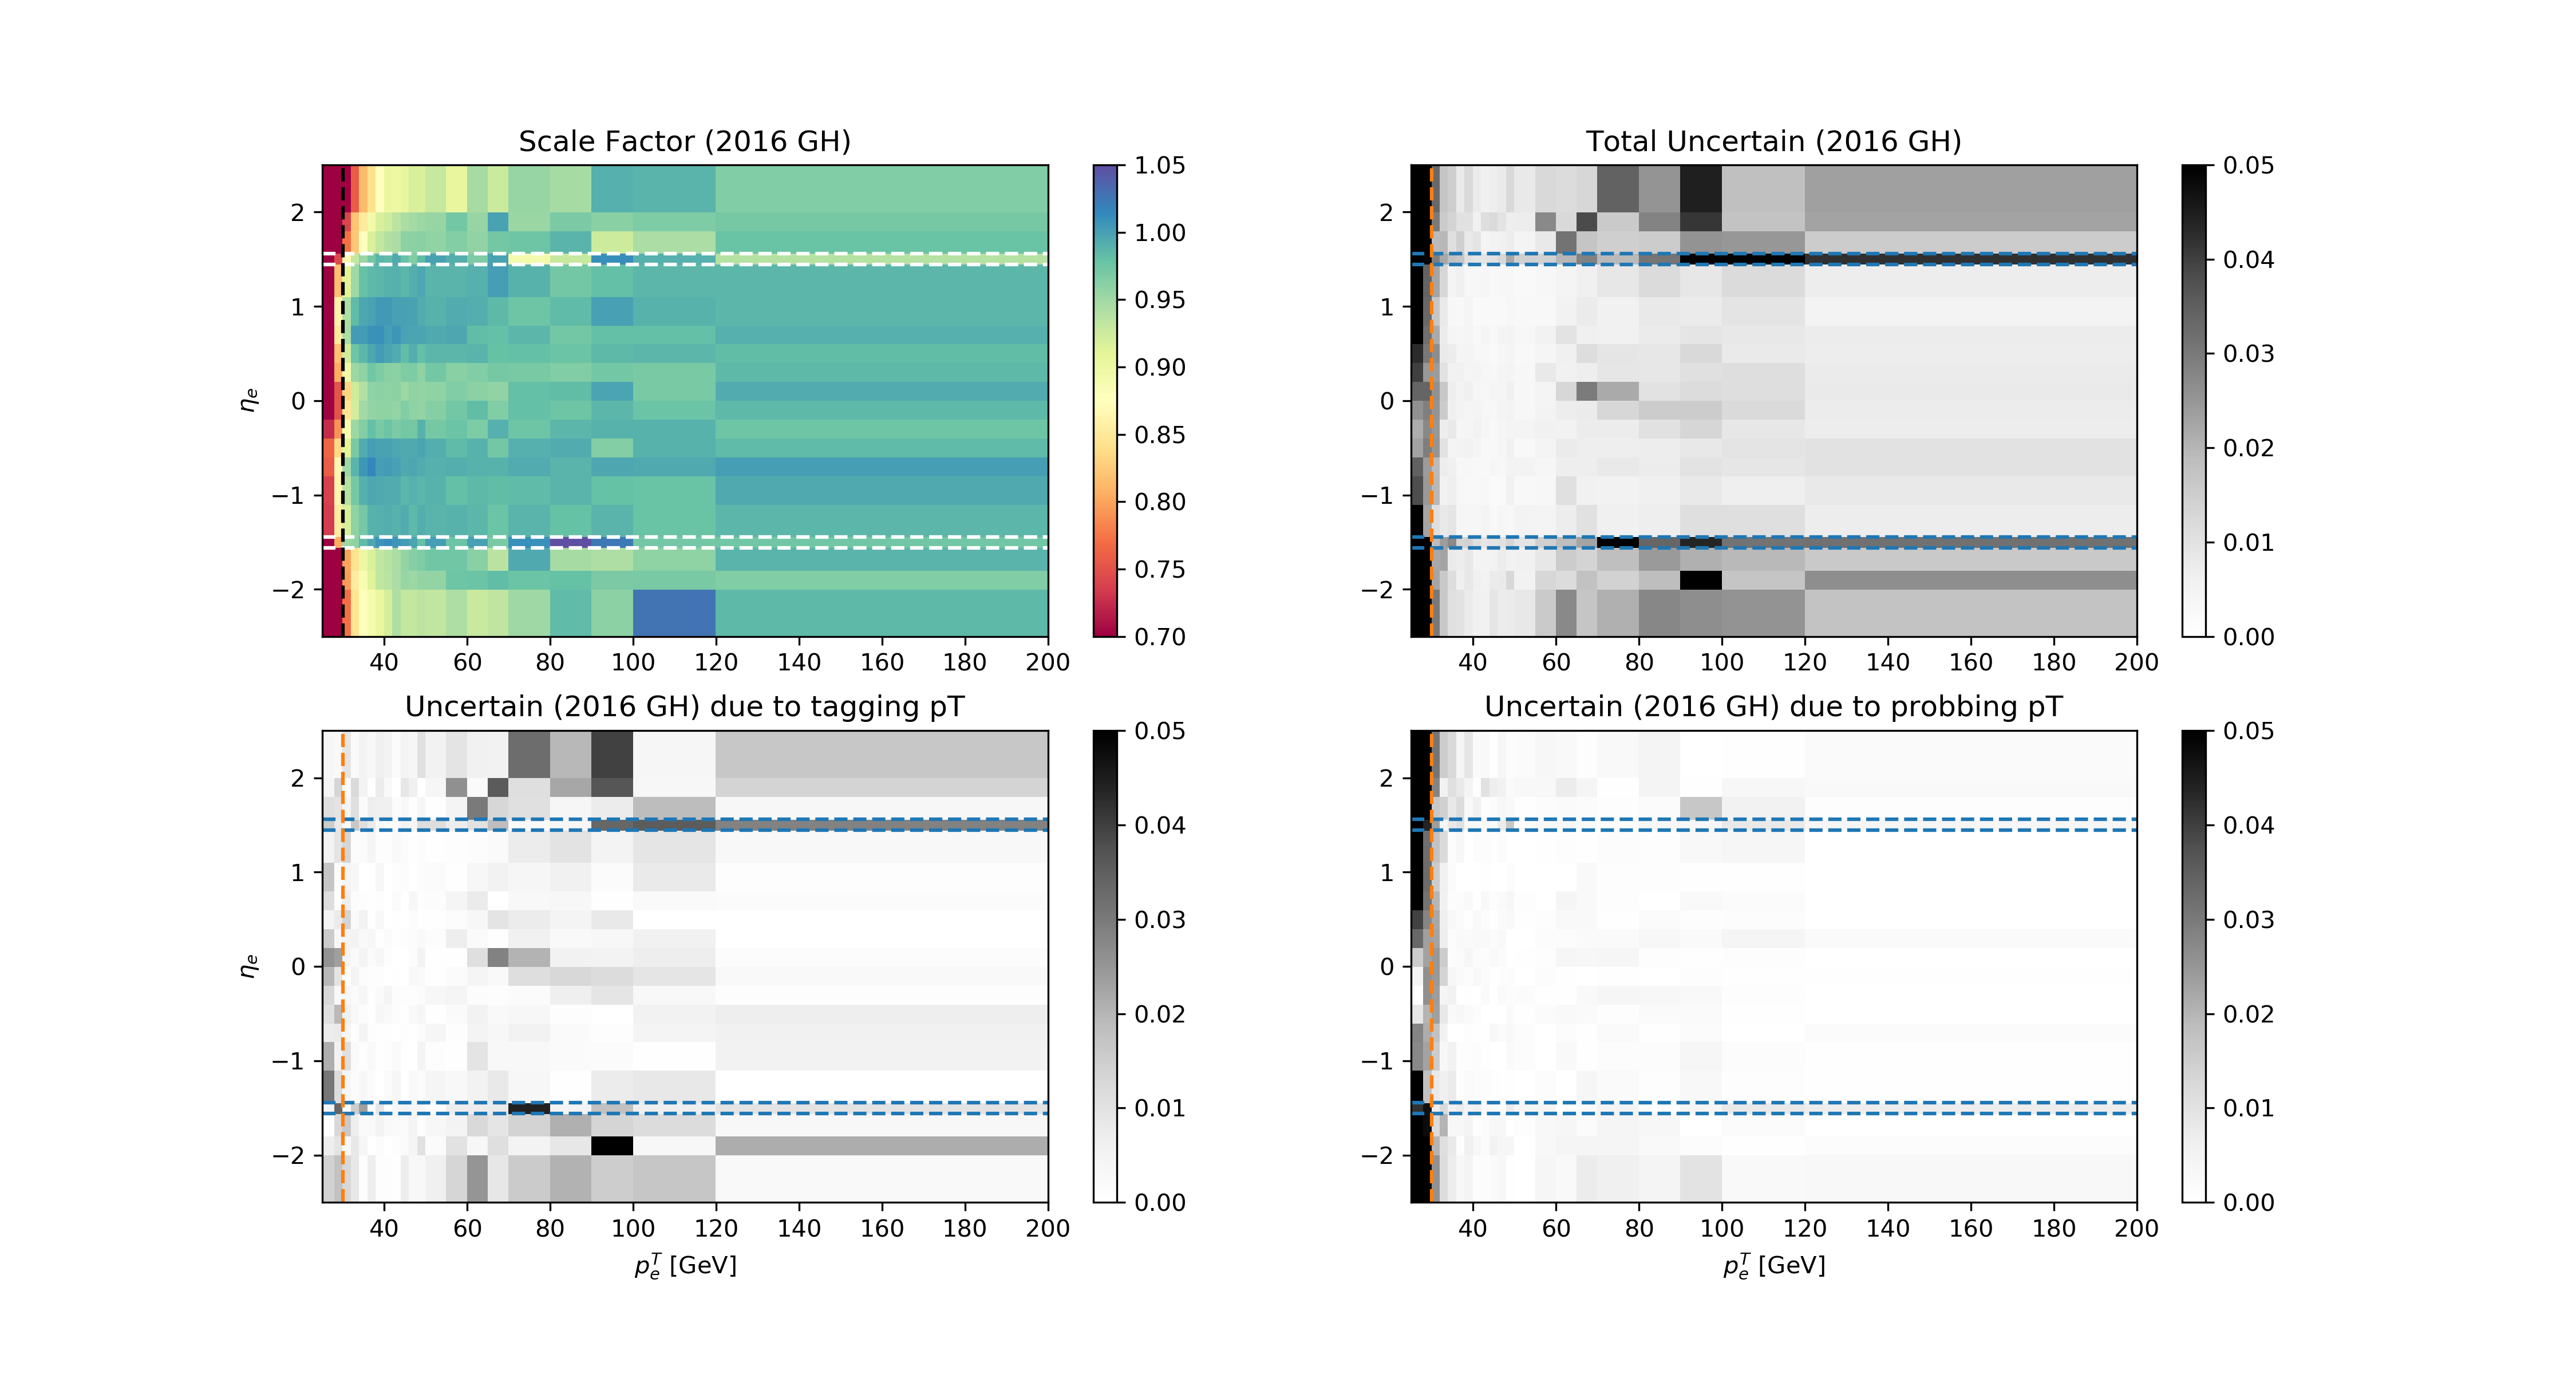
\includegraphics[width=0.99\textwidth]{chapters/Appendix/sectionEleTrigger/figures/result_GH.png}
    
    \caption{SF and the associated uncertainties in the 2016 GH.}
    \label{fig:eTrSF_err_GH}
\end{figure}

\FloatBarrier
